\documentclass[11pt]{article}

\usepackage{amsmath}
\usepackage{amssymb}
\usepackage{palatino}
\usepackage[usenames,dvipsnames]{xcolor}
\usepackage{tikz}
\usepackage[retainorgcmds]{IEEEtrantools}
\usetikzlibrary{arrows}
\newcommand*\circled[1]{\tikz[baseline=(char.base)]
	{
		\node[shape=circle, draw, inner sep=1.6pt] (char) {#1};
	}
}

\begin{document}

\centerline{	
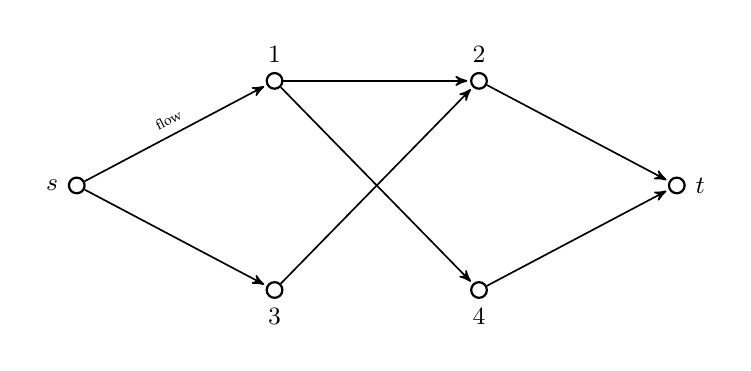
\begin{tikzpicture}[point/.style={circle, thick, draw=black, inner sep=2pt},
					post/.style={->, shorten >=1pt, >=stealth', semithick}]
	\matrix[column sep=22mm, row sep=10mm, ampersand replacement = \&]{
	 \&\node[point, label=above:\small{$1$}] (1) {}; \& \node[point, label=above:\small{$2$}] (2) {};\&\\
	 \node[point, label=left:\small{$s$}] (s) {};\& \& \&\node[point, label=right:\small{$t$}] (t) {};\\
	 \&\node[point, label=below:\small{$3$}] (3) {}; \& \node[point, label=below:\small{$4$}] (4) {};\&\\
	};
	\draw[post] (s) -- node[sloped, above] {\tiny{flow}} (1);
	\draw[post] (s) -- node[sloped, above] {}  (3);
	\draw[post] (1) -- node[sloped, above] {} (2);
	\draw[post] (1) -- node[near end, sloped, above] {} (4);
	\draw[post] (3) -- node[near end, sloped, above] {} (2);
	\draw[post] (2) -- node[sloped, above] {} (t);
	\draw[post] (4) -- node[sloped, above] {} (t);
\end{tikzpicture}
}

\end{document}